\section{How to visualize a PDB file in VMD software package}

The PDB file written by JETSPIN can be easily visualized in VMD software
package. The first step is to download and install VMD which can be
found at website: \href{http://www.ks.uiuc.edu/Research/vmd/}{http://www.ks.uiuc.edu/Research/vmd/}.
As VMD is installed, the PDB file can be opened using VMD: \textquotedbl{}vmd
frame000001.pdb\textquotedbl{} in the terminal or click on \textquotedbl{}file\textquotedbl{}
in the main white box and then on \textquotedbl{}load molecule\textquotedbl{}
(see Fig \ref{fig:vmd1}), browse for your PDB file frame000001.pdb
and load it. In order to load the topological structure of the jet,
it is possible to load the PSF file written by JETSPIN alongside the
PDF file: right click on the just uploaded file (e.g. \textquotedbl{}frame000001.pdb\textquotedbl{})
in the white box in the middle of the \textquotedbl{}MD Main\textquotedbl{}
window, and select \textquotedbl{}Load Coordinates into Molecule\textquotedbl{}
pull-down menu option (see Fig \ref{fig:vmd2}). Hence, browse for
the PSF file (frame000001.psf) defining the bonds for each pair of
consecutive jet beads, and load it. Finally, the jet will be displayed
in the graphics window.

\begin{figure}
\begin{centering}
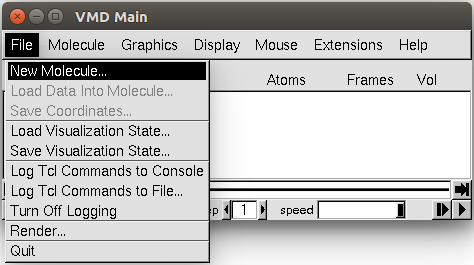
\includegraphics[scale=0.5]{vmd1}
\par\end{centering}
\caption{Snapshot of the main white box of VMD.}

\label{fig:vmd1}
\end{figure}

\begin{figure}
\begin{centering}
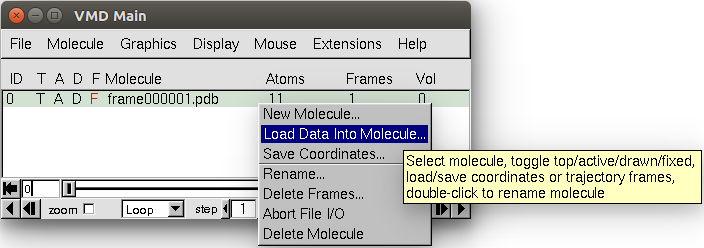
\includegraphics[scale=0.5]{vmd2}
\par\end{centering}
\caption{Snapshot of the \textquotedbl{}Load Coordinates into Molecule\textquotedbl{}
selection in VMD.}

\label{fig:vmd2}
\end{figure}
